%%%%%%%%%%%%%%%%%%%%%%%%%%%%%%%%%%%%%%%%%%%%%%%%%%%%%%%%%%%%%%%%%%%%%%%%%%%%%%%%
%2345678901234567890123456789012345678901234567890123456789012345678901234567890
%        1         2         3         4         5         6         7         8
\documentclass[letterpaper, 10pt, conference]{ieeeconf}  % Comment this line out if you need a4paper
%\documentclass[a4paper, 10pt, conference]{ieeeconf}      % Use this line for a4 paper
\IEEEoverridecommandlockouts                              % This command is only needed if 
                                                          % you want to use the \thanks command
\overrideIEEEmargins     
% Needed to meet printer requirements.
\usepackage{url}
\usepackage{svg}
\usepackage[backend=biber,
            hyperref=true,
            url=false,
            isbn=false,
            doi=false,
            backref=false,
            style=ieee,
            natbib=true,%compatibility aliases
            mincitenames=1,
            maxcitenames=1,
            citestyle=numeric-comp,
            sorting=nyt,%none
            block=none]{biblatex}
            
\addbibresource{example.bib}
% \DeclareUnicodeCharacter 
%\usepackage{multicol,multirow}
\usepackage{amsmath,amssymb}
\usepackage{graphicx,color}
\usepackage{adjustbox}
\usepackage{booktabs}
\usepackage{multirow}
\usepackage{verbatim}
\usepackage{multicol}
\usepackage{subfig}
\usepackage{caption}
\usepackage{float}
\captionsetup[figure]{font=footnotesize,labelfont=footnotesize}
\captionsetup[table]{font=footnotesize,labelfont=footnotesize}
\usepackage{xspace}
\usepackage{gensymb}
\usepackage{marginnote}
\usepackage{siunitx} % Daniel: added based on Jeff's prior papers. (needs to be paired with next line :) -Jeff)
\sisetup{detect-all} % <-- fixes fonts in siunitx
\usepackage{pythonhighlight} % try to highlight python code
\graphicspath{{figures/}}
\newcommand{\ba}{\mathbf{a}}
\newcommand{\bd}{\mathbf{d}}
\newcommand{\bm}{\mathbf{m}}
\newcommand{\bo}{\mathbf{o}}
\newcommand{\br}{\mathbf{r}}
\newcommand{\bs}{\mathbf{s}}
\newcommand{\bx}{\mathbf{x}}
\newcommand{\bu}{\mathbf{u}}
\newcommand{\state}{\mathbf{s}}
\newcommand{\vmax}{v_{\rm max}}
% Neat, and useful to make sure puntuation is correct, but let's not italicize i.e. and e.g.,
% See https://www.grammarly.com/blog/know-your-latin-i-e-vs-e-g/
% https://www.quora.com/Should-I-italicize-e-g-and-i-e
% \newcommand{\ie}{\emph{i.e.,}\xspace}
% \newcommand{\eg}{\emph{e.g.,}\xspace}
\newcommand{\ie}{i.e.,\xspace}
\newcommand{\eg}{e.g.,\xspace}

% Daniel: for ease of changing names.
\newcommand{\dtune}{\mathcal{D}_\textrm{tune}}
\newcommand{\dsim}{\mathcal{D}_\textrm{sim}}
\newcommand{\dreal}{\mathcal{D}_\textrm{phys}}
\newcommand{\pitune}{\pi_\textrm{R2S2R}}
\newcommand{\pisim}{\pi_\textrm{SD}}
\newcommand{\pireal}{\pi_\textrm{RD}}
\newcommand{\polarcasting}{Cast and Pull\xspace}
% \newcommand{\dphys}{\mathcal{D}_{\textrm{p}}}
% \newcommand{\dsim}{\mathcal{D}_{\textrm{s}}

% Daniel: for better argmax and argmin.
\DeclareMathOperator*{\argmax}{arg\,max}
\DeclareMathOperator*{\argmin}{arg\,min}
\DeclareMathOperator*{\minimize}{minimize}

%\usepackage[dvipsnames]{xcolor} % Daniel: was causing an issue and doesn't seem necessary ?
\usepackage{pifont}
\newcommand{\cmark}{\textcolor[HTML]{59a14f}{\ding{51}}}%
\newcommand{\xmark}{\textcolor[HTML]{e15759}{\ding{55}}}%


\setlength{\marginparwidth}{.5in}

% Daniel: feel free to add your names with your favorite color!
% Wrap around the shared "\remark" command for consistency, and to make it easy to turn all remarks off by defining an empty command. -Jeff
% Thanks! -Daniel (do we want \bf, some had it, some did not?)  (We don't need bf for now -Daniel)
% Heh... except KG ones :)
\newcommand{\remark}[3]{{\color{#2}[#1: #3]}}
% \renewcommand{\remark}[3]{} % To disable all remarks, uncomment
\newcommand{\daniel}[1]{\remark{Daniel}{blue}{#1}}
\newcommand{\jonathan}[1]{\remark{Jonathan}{cyan}{#1}}
\newcommand{\harry}[1]{\remark{Harry}{green}{#1}}
\newcommand{\Vincent}[1]{\remark{Vincent}{purple}{#1}}
\newcommand{\Lawrence}[1]{\remark{Lawrence}{orange}{#1}}
\definecolor{britishracinggreen}{rgb}{0.23, 0.53, 0.19}
\newcommand{\raven}[1]{\remark{Raven}{britishracinggreen}{#1}}
\newcommand{\jeffi}[1]{\remark{JI}{red}{#1}}
\definecolor{turquoise}{rgb}{0.25, 0.88, 0.82}
\newcommand{\ale}[1]{\remark{Alejandro}{turquoise}{#1}}

\newcommand{\KG}[1]{\remark{KG}{magenta}{#1}}

\definecolor{navy}{rgb}{0,0,0.5}
\newcommand{\NEW}[1]{{\color{navy} #1}}


\usepackage[font={small}]{caption}

% Daniel: argh I thought this would avoid capital 'TABLE' text but doesn't seem to be working...
\def\tablename{Table}


\title{\LARGE \bf
Real2Sim2Real: Self-Supervised Learning of Physical \\ Single-Step Dynamic Actions for Planar Robot Casting
}

\author{Vincent Lim$^{1,*}$, Huang Huang$^{1,*}$, Lawrence Yunliang Chen$^{1}$, Jonathan Wang$^{1}$, \\  Jeffrey Ichnowski$^{1}$, Daniel Seita$^{1}$, Michael Laskey$^2$, Ken Goldberg$^1$% <-this % stops a space
\thanks{*Equal contribution.}% <-this % stops a space
\thanks{$^{1}$The AUTOLab at UC Berkeley (automation.berkeley.edu).}%
\thanks{$^{2}$Toyota Research Institute, CA, USA.}
\thanks{Correspondence to: {\tt\scriptsize \{vincentklim, huangr\}@berkeley.edu}}
}
\begin{document}


\maketitle
\thispagestyle{empty}
\pagestyle{empty}


%%%%%%%%%%%%%%%%%%%%%%%%%%%%%%%%%%%%%%%%%%%%%%%%%%%%%%%%%%%%%%%%%%%%%%%%%%%%%%%%
\begin{abstract}
This paper introduces the task of {\em Planar Robot Casting (PRC)}: where one planar motion of a robot arm holding one end of a cable causes the other end to slide across the plane toward a desired target. PRC allows the cable to reach points beyond the robot workspace and has applications for cable management in homes, warehouses, and factories. To efficiently learn a PRC policy for a given cable, we propose {\em Real2Sim2Real}, a self-supervised framework that automatically collects physical trajectory examples to tune parameters of a dynamics simulator using Differential Evolution, generates many simulated examples, and then learns a policy using a weighted combination of simulated and physical data. We evaluate Real2Sim2Real with three simulators, Isaac Gym-segmented, Isaac Gym-hybrid, and PyBullet, two function approximators, Gaussian Processes and Neural Networks (NNs), and three cables with differing stiffness, torsion, and friction. Results with 240 physical trials suggest that the PRC policies can attain median error distance (as \% of cable length) ranging from 8\% to 14\%, outperforming baselines and policies trained on only real or only simulated examples.
% Results with 5 trials $\times$ 16 held-out test targets $\times$ 3 cables $=$ 240 physical trials suggest that the PRC policies can attain median error distance (as \% of cable length) ranging from 8\% to 14\%, outperforming baselines and policies trained on only real or only simulated examples.
Code, data, and videos are available at \url{https://tinyurl.com/robotcast}.
\end{abstract}


\section{Introduction}\label{sec:intro}

Manipulation of deformable objects using a single parameterized dynamic action can be useful for tasks such as fly fishing, lofting a blanket, and playing shuffleboard. Such tasks take as input a desired final state and output one parameterized open-loop dynamic robot action which produces a trajectory toward the final state.  This is especially challenging for long-horizon trajectories with complex dynamics involving friction. Although there is substantial research on learning ballistic throwing or hitting motions for rigid objects~\cite{lynch1999dynamic,zeng_tossing_2019}, there is less research into learning dynamic motions to manipulate deformable objects such as cables and fabrics. 
%in the presence of friction and varying stiffness.   
Dynamics modeling in these contexts is challenging due to uncertainty in deformability, elasticity, and friction during the object's motion. When computing a single action in this setting (without feedback control), the complexities of state estimation and dynamics modeling are compounded by the long duration for which the system evolves after the robot action. Simulation is often used as an alternative to collecting physical examples, which can be time-consuming and hazardous. However, overcoming the simulation to reality (Sim2Real) gap is a long-standing problem in robotics~\cite{rss_workshop, reality_gap_1995,mahler2017dexnet,domain_randomization}, and is particularly challenging for deformable objects in uncertain dynamic environments.

\begin{figure}[t]
\center
\includegraphics[width=0.49\textwidth]{figures/teaser_v09.jpg}
\caption{
In \emph{Planar Robot Casting} (PRC), a single dynamic planar motion of a robot wrist holding one end of a cable causes the other end of the cable to slide across the plane and stop near a desired target point,  which may lie outside the robot workspace. (A) shows a side view of a UR5 robot with cable and planar workspace, (B) illustrates test performance on Cable 1 for 5 trials (dots) on 16 targets (stars). The gold inner sector represents the robot workspace, while the grey outer sector represents the reachable workspace of the cable. (C,D) each show five superimposed overhead views of the robot and cable with associated target points after PRC actions with the learned policy, in (C) an example with low error and in (D) an example with high error in endpoint position. 
}
\vspace{-16pt}
\label{fig:teaser}
\end{figure}

In this paper, we introduce \emph{Planar Robot Casting} (PRC), where a robot arm dynamically manipulates a cable through 2D space, as illustrated in Fig.~\ref{fig:teaser}. We use the generic term \emph{cable} to refer to any 1D deformable object with low stiffness, such as cables, ropes, and threads. We propose {\em Real2Sim2Real}, a self-supervised robot learning framework that starts by efficiently collecting a small number of physical examples, uses them to tune a simulator, and then uses a combination of physical and simulated examples to train policies for PRC. This paper makes four contributions:

\begin{enumerate}
    \item Real2Sim2Real, a three-step robot learning framework for single-step dynamic actions executed in real environments.
    \item A formulation of the Planar Robot Casting (PRC) problem, with an automated reset motion and parameterized one-step action space that can reach outside of the reachable area of the robot. 
    \item  A physical implementation of PRC using a UR5 robot, and three simulation models of PRC: NVIDIA Isaac Gym \emph{segmented}, Isaac Gym \emph{hybrid}, and PyBullet. Parameter estimation using Differential Evolution~\cite{storn1997differential,2020SciPy-NMeth} with associated code and datasets from 64,350 simulated experiments and 2,076 physical experiments with 3 distinct cables.
    \item An application of Real2Sim2Real to PRC, with results suggesting that Real2Sim2Real can efficiently learn PRC control policies that reach target positions within median error of 14\% of cable length, even when targets are outside the reachable workspace of the robot.
\end{enumerate}

\section{Related Work}\label{sec:rw}

\subsection{Deformable 1D Object Manipulation}

Manipulation of 1D deformable objects such as cables has a long history in robotics; see~\citet{manip_deformable_survey_2018} for a recent survey. Some representative applications include surgical suturing~\cite{robot_heart_surgery_2006,suturing_autolab_2016}, knot-tying~\cite{van_den_berg_2010,case_study_knots_1991,knot_planning_2003,tying_precisely_2016}, untangling ropes~\cite{rope_untangling_2013,grannen2020untangling}, deforming wires~\cite{wire_insertion_1997}, inserting cables into receptacles~\cite{tight_tolerance_insertion_2015,tactile_cable_2020}, and playing diabolo~\cite{diabolo_2020}.  

There is recent interest in using learning-based techniques for manipulating cables, often with pick-and-place actions and quasistatic dynamics, so that the robot deforms the cable while allowing it to settle between actions. This can be combined with learning from demonstrations~\cite{zeng_transporters_2020,seita_bags_2021} and self-supervised learning~\cite{nair_rope_2017,ZSVI_2018}.
Prior work has also used quasistatic simulators~\cite{corl2020softgym} to train cable manipulation policies using reinforcement learning (RL) for transfer to physical robots~\cite{lerrel_2020,yan_fabrics_latent_2020}. 
However, as we show in Sec.~\ref{sec:experiments}, there are limits in the free-end reachability of such quasistatic procedures, motivating high-speed, dynamic motions.


\subsection{Simulator Tuning for Sim2Real}

Sim2Real transfer has emerged as an effective technique wherein a robot can learn a policy in simulation and transfer it to the real world, which can suffer from the mismatch between simulation and real~\cite{reality_gap_1995}. One option for Sim2Real is to perform system identification~\cite{sys_id} to tune a simulator to match real-world data, but this may be challenging with the infinite-dimensional configuration spaces of cables.
An alternative is to use domain randomization over vision~\cite{domain_randomization,cad2rl} or dynamics~\cite{dynamics_randomization_2018} parameters in simulation.
A drawback is that too much randomization can hinder policy training~\cite{sim2real_deform_2018} and the randomization range needs to be hand tuned.
% that researchers must estimate suitable ranges for parameters to randomize. 
This has motivated work on interleaving policy training using RL in simulation and tuning simulators with real-world data~\cite{closing_sim2real_2019,auto-tune_2021}. Recently, Chang and Padir~\cite{sim2real2sim_2020} proposed a Sim2Real2Sim pipeline for cable unplugging where the Sim2Real step determines grasp points, and the Real2Sim step uses sensors to update a cable model in simulation.
Similarly, we tune a simulator, but do not require repeated iterations of collecting real-world data with simulator tuning, and we train policies using supervised learning and do not need to use potentially brittle RL algorithms~\cite{SpinningUp2018,how_to_train_rl}. Unlike Chang and Padir, we do not require cable sensors and we use the tuned simulator to improve the performance of the physical robot.
%While these methods rely on a feedback loop, we focus on a single-action task.
%\jeffi{TODO: make sure to contrast differences: single-action vs RL, long-horizon predictions in simulation (not just single time-step), no-feedback during evolution of system}

\subsection{Dynamic Manipulation}

% Daniel: I'd classify the Lynch+Mason paper as a deep theoretical study + method, so I summarized it as 'study'. Also, after searching, I realize those two have ANOTHER paper from 1993 (!), with the literal title 'Dynamic Manipulation.'
In dynamic manipulation, a robot executes rapid actions to move objects to desired configurations~\cite{lynch_mason_1993}. 
In early work, Lynch and Mason~\cite{lynch1999dynamic} study planar dynamic manipulation primitives such as snatching, throwing, and rolling, and~\citet{ruiz2011fast} build a physics-based model of pushing actions so that a robot can slide objects into a desired pose.
More recent work has introduced robots that can catch items by predicting item trajectories~\cite{catching_2014}, toss arbitrary objects via self-supervised learning~\cite{zeng_tossing_2019}, 
%control the motion of rolling bodies~\cite{woodruff2020motion}, 
and swing items upwards using tactile feedback~\cite{swingbot_2020}.
As with these works, we use dynamic motions, but focus specifically on cable manipulation. Furthermore, we use a tuned simulator to accelerate learning and do not require tactile sensing.


\subsection{Dynamic Manipulation of Deformable Objects}

Researchers have developed several analytic physics models to describe the dynamics of moving cables. For example,~\citet{fly_fishing_2004} present a 2D dynamic model of fly fishing. They model the fly line as a long elastica and the fly rod as a flexible Euler-Bernoulli beam, and propose a system of differential equations to predict the movement of the fly line in space and time. 
In contrast to continuum models,~\citet{wang2011analysis} propose using a finite-element model to represent the fly line by a series of rigid cylinders that are connected by massless hinges. In contrast to these works, we evaluate on physical robots.

For robotic dynamic-cable manipulation,~\citet{dynamic_knotting_2010,yamakawa2012simple,high_speed_knotting_2013,one_hand_knotting_tactile_2007} 
% show that a high-speed manipulator can tie knots using snapping motions. They
simplify the modeling of cable deformation by assuming each cable component follows the robot end-effector motion with constant time delay. %\jeffi{Note how Yamakawa work does not address the complex state-estimation and dynamics required for casting?}
\citet{kim2016using} study a mobile robot system with a cable attached as a tail that can strike objects.
%This high-speed setting allows them to construct primitive motions that exploit the dynamics of the tail. 
They use a Rapidly-exploring Random Tree (RRT)~\cite{RRT_2001} and a particle-based representation to address the uncertainty in state transition. In contrast, we aim to control cables for tasks in which we may be unable to rely on assumptions in~\cite{yamakawa2012simple,kim2016using} for cable motion.


% Daniel: please us this figure:
% https://docs.google.com/drawings/d/1kao1uhGFjieGHyiPboKGiYFg6oXGlXv6Z3Q0Mx_M_xE/edit?usp=sharing for the old figure
% Vincent: use this link for the new figure: (v01)
% https://docs.google.com/drawings/d/1pU0LzYIhabU_R34ZbvAxZbv_iGznAzZ9alFwL1ZuP_s/edit?usp=sharing
% pipeline-v02 ("column-width"
% https://docs.google.com/drawings/d/1J3H03YccTQC5hLcF_g3RAFej6BfQx7ja95eiIz6P8ZA/edit?usp=sharing
% pipeline-v03 (use 2x2 grids)
% https://docs.google.com/drawings/d/1le71m1Ru_uXHIOzYWW0fZnpuneBFP_z5TRzrEN_hbSU/edit?usp=sharing
% pipeline-v04 (removed reset)
% https://docs.google.com/drawings/d/1S8EZQ_f4eoFrLjH6W2OwAGHq1uooV4qZIe7_gODDLtw/edit?usp=sharing
% pipeline-v08
%https://docs.google.com/drawings/d/1sy5zXH3d0QH8egsFlE0dh6WAslKkTl7RbYybDTg6pTY/edit
\begin{figure*}[t]
\center
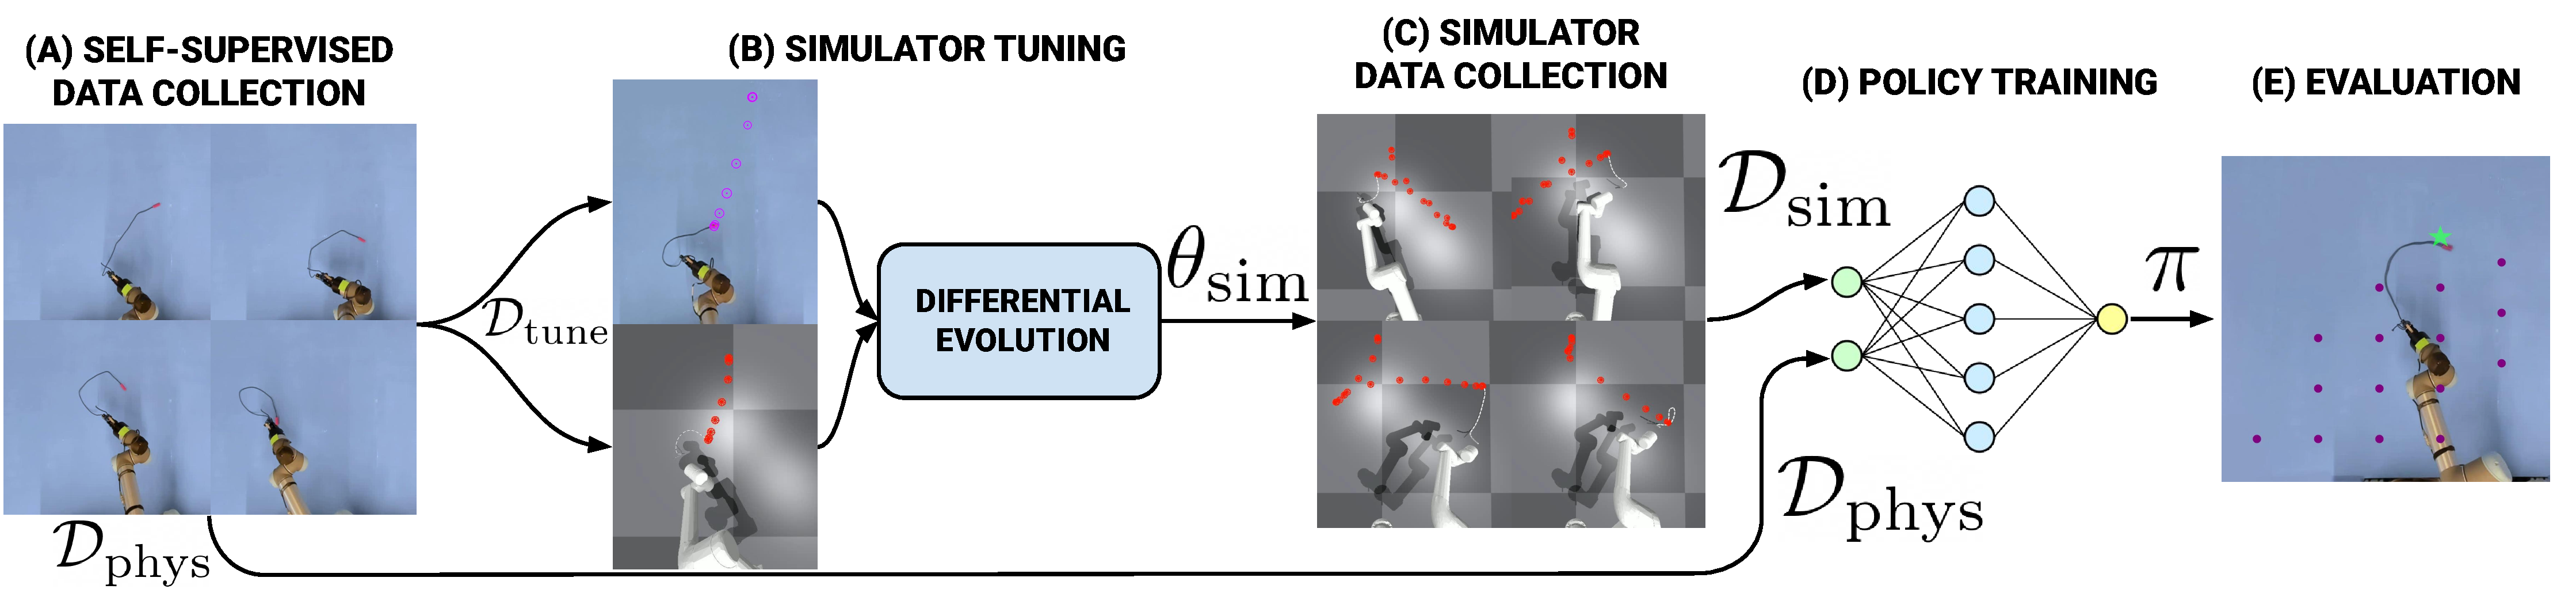
\includegraphics[width=1.00\textwidth]{figures/pipeline-v08.pdf}
\caption{The \emph{Real2Sim2Real} pipeline for PRC. We collect a physical dataset $\dreal$ (A) in a self-supervised manner. We subsample $\dreal$ to generate $\dtune$, and use it to tune simulation parameters so that its trajectories match real trajectories using Differential Evolution (B), then use the tuned simulator to generate a large dataset $\dsim$ (C). We use a weighted combination of $\dsim$ and $\dreal$ to train the policy (D) and evaluate the policy in real (E).
% for pipeline-v03 and below
% The \emph{Real2Sim2Real} pipeline for the PRC task. We develop a reset motion (A) to enable self-supervised data collection and collect a physical dataset $\dreal$ (B). We subsample $\dreal$ to generate $\dtune$ and use $\dtune$ to tune the simulation parameters to match real using Differential Evolution (C), then use the tuned simulation parameters to generate a large dataset $\dsim$ (D). We use a weighted combination of $\dsim$ and $\dreal$ to train the policy (E) and evaluate the policy in real (F).
}
\vspace*{-10pt}
\label{fig:process}
\end{figure*}

In closely related prior work,~\citet{harry_rope_2021} propose a self-supervised learning technique for dynamic manipulation of fixed-end cables.
% for vaulting, knocking, and weaving. 
% They parameterize actions by computing a motion using a quadratic program and learning the apex point of the trajectory. 
In contrast, we use free-end cables. \citet{zimmermanndynamic} study the dynamic manipulation of deformable beams and cloth in the free-end setting. They model elastic objects using the finite-element method~\cite{bathe2006finite} and use optimal control techniques for trajectory optimization. 
% They study whipping a beam so that its free end hits a predefined target with maximum speed. % and laying a cloth on the table.
The simulated motions perform well in real for simple dynamical systems %such as a pendulum, 
but performance deteriorates for complex soft bodies due to the reality gap. %mismatch between simulation and the real world. 
We develop a learned, data-driven approach for robotic manipulation of free-end cables and focus on PRC.
\citet{9561766} develop six customizable benchmark simulation environments for 1D deformable objects, but use an commercial closed-source physics engine. We use easily-accessible physics engines to create dynamic simulation environments. 



\section{Problem Statement}\label{sec:PS}

In Planar Robot Casting, a robot gripper holds a cable at one endpoint and swings it along a planar surface with a single continuous motion so that the other endpoint comes to rest at a target $\state_d$.
The held cable endpoint is at polar coordinate ${\state=(r, \theta)}$, with the robot base at the origin.
%A policy $\pi$, when given the desired target ${\state_d}$ for the endpoint, outputs a dynamic arm action ${\ba}$ parametrized by a vector of six dimensions as in Section~\ref{ssec:action} that moves the endpoint to $\state_f$. 
The objective is to find a per-cable policy $\pi$ that minimizes the expected error $||\state_{f, c}-\state_{d, c}||_2$, where $\state_{f, c}$ is the final state and $\state_{d, c}$ is $\state_d$ in Cartesian coordinates. We assume that the $\state_d$ is reachable by the cable endpoint (see Fig.~\ref{fig:teaser}).
% for $\state_d$ from the feasible set defined as the half-circle with a radius being the sum of the cable length and radius of the robot work-space (see Fig.~\ref{fig:teaser}).


\section{Method} \label{sec:approach}

To learn a policy that accounts for variations in cable properties such as mass, stiffness, and friction, % require different policies. To learn a different policy for each cable, 
we propose the \emph{Real2Sim2Real} (R2S2R) framework (Fig.~\ref{fig:process}) and apply it to PRC. To support this framework, we define a reset procedure to bring the system into a consistent starting state and a parameterized trajectory function that generates a dynamic arm action. R2S2R first autonomously collects physical trajectories, then tunes a simulator to match the physical environment and generate simulated trajectories. %We evaluate three simulation models and two tuning algorithms
Finally, R2S2R uses a weighted combination of the simulated and physical datasets to train a policy.
%We aim to find the best-performing simulation model and tuning algorithm, and evaluate the R2S2R framework on three different cables.


\subsection{Reset Procedure}\label{ssec:resets}

To automate data collection and bring the cable into a consistent starting state before each action, we define a 5-step reset procedure, in which the robot
%
%\begin{enumerate}
%\item 
(1) lifts the cable up with the free-end touching the surface to prevent the cable from dangling;
%\item
(2) continues to lift the cable such that the free-end is just above the surface;
%\item
(3) hangs still for 3 seconds to stabilize; 
%\item
(4) swings the cable out of the plane, so that the cable straightens along the center axis of the surface and lands with its endpoint far from the robot base; and
(5) slowly pulls the cable towards the robot to the reset position $(r_0, 0)$. %  \jeffi{This doesn't match with $(r_0, \theta_0)$ in the action parameterization.  Which is it?} 
%\Lawrence{From our IROS reviewer: ``What is the reset position? How is it chosen and how is it different from the origin of the polar coordinate frame discussed in V B? From Fig 4F and Fig 5, it seems the ee 2D locations in the reset position and the polar coordinate frame locations are the same.''}
%\end{enumerate}
The reset motion is designed to minimize empirical uncertainty in the reset state, so we assume the start state to be consistent across trajectories. The project website illustrates the reset procedure.

% Daniel: please edit with:
% https://docs.google.com/drawings/d/1BokQw642ME_br0toxppAit2yO8ojL-5BqMuFE0mhYVY/edit?usp=sharing
\begin{figure}[t]
\center
% 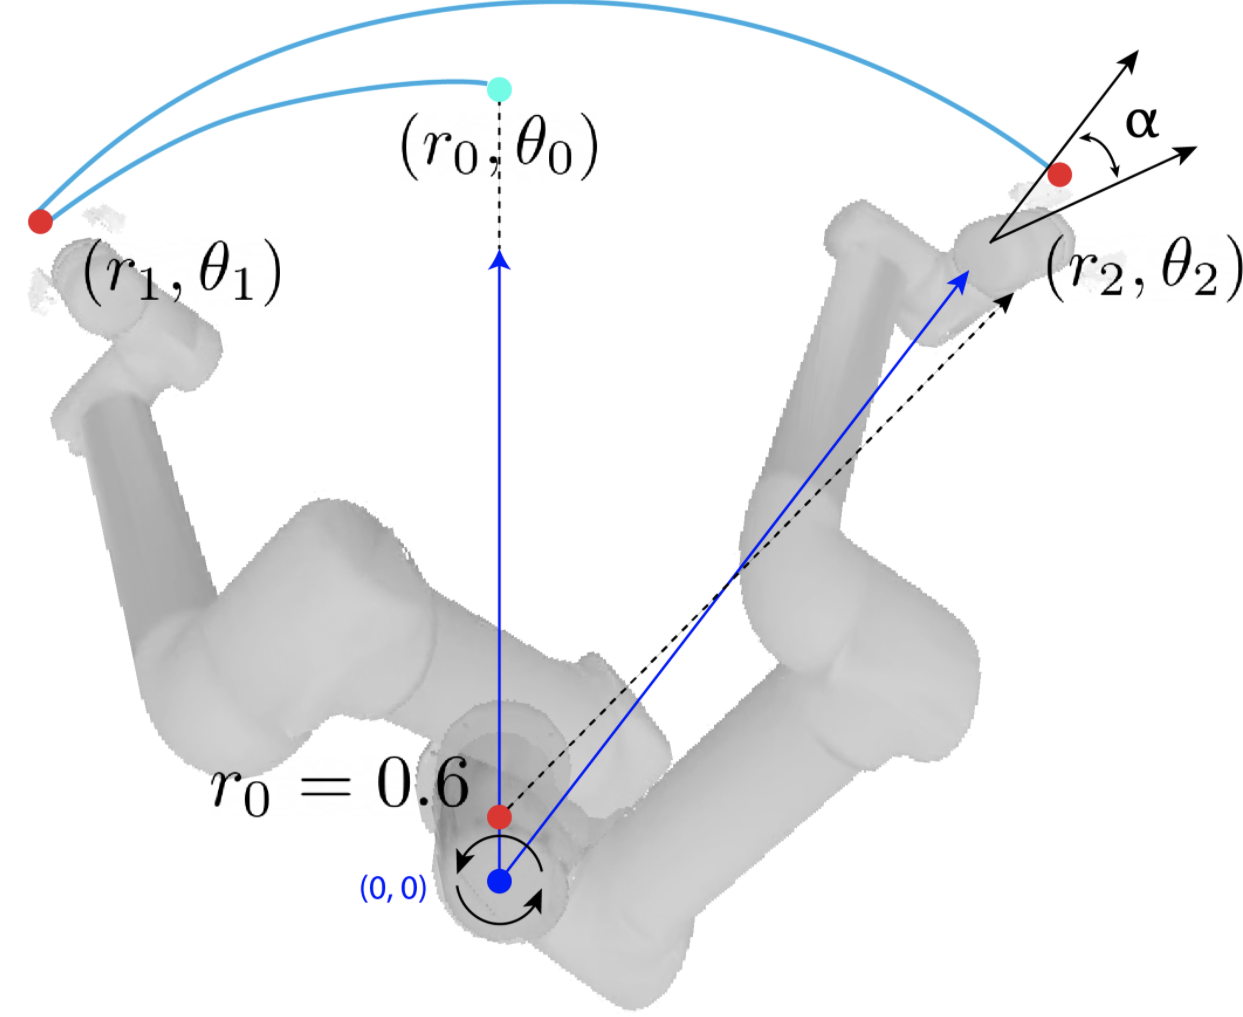
\includegraphics[width=0.33\textwidth]{figures/splinenew_truncated.png}
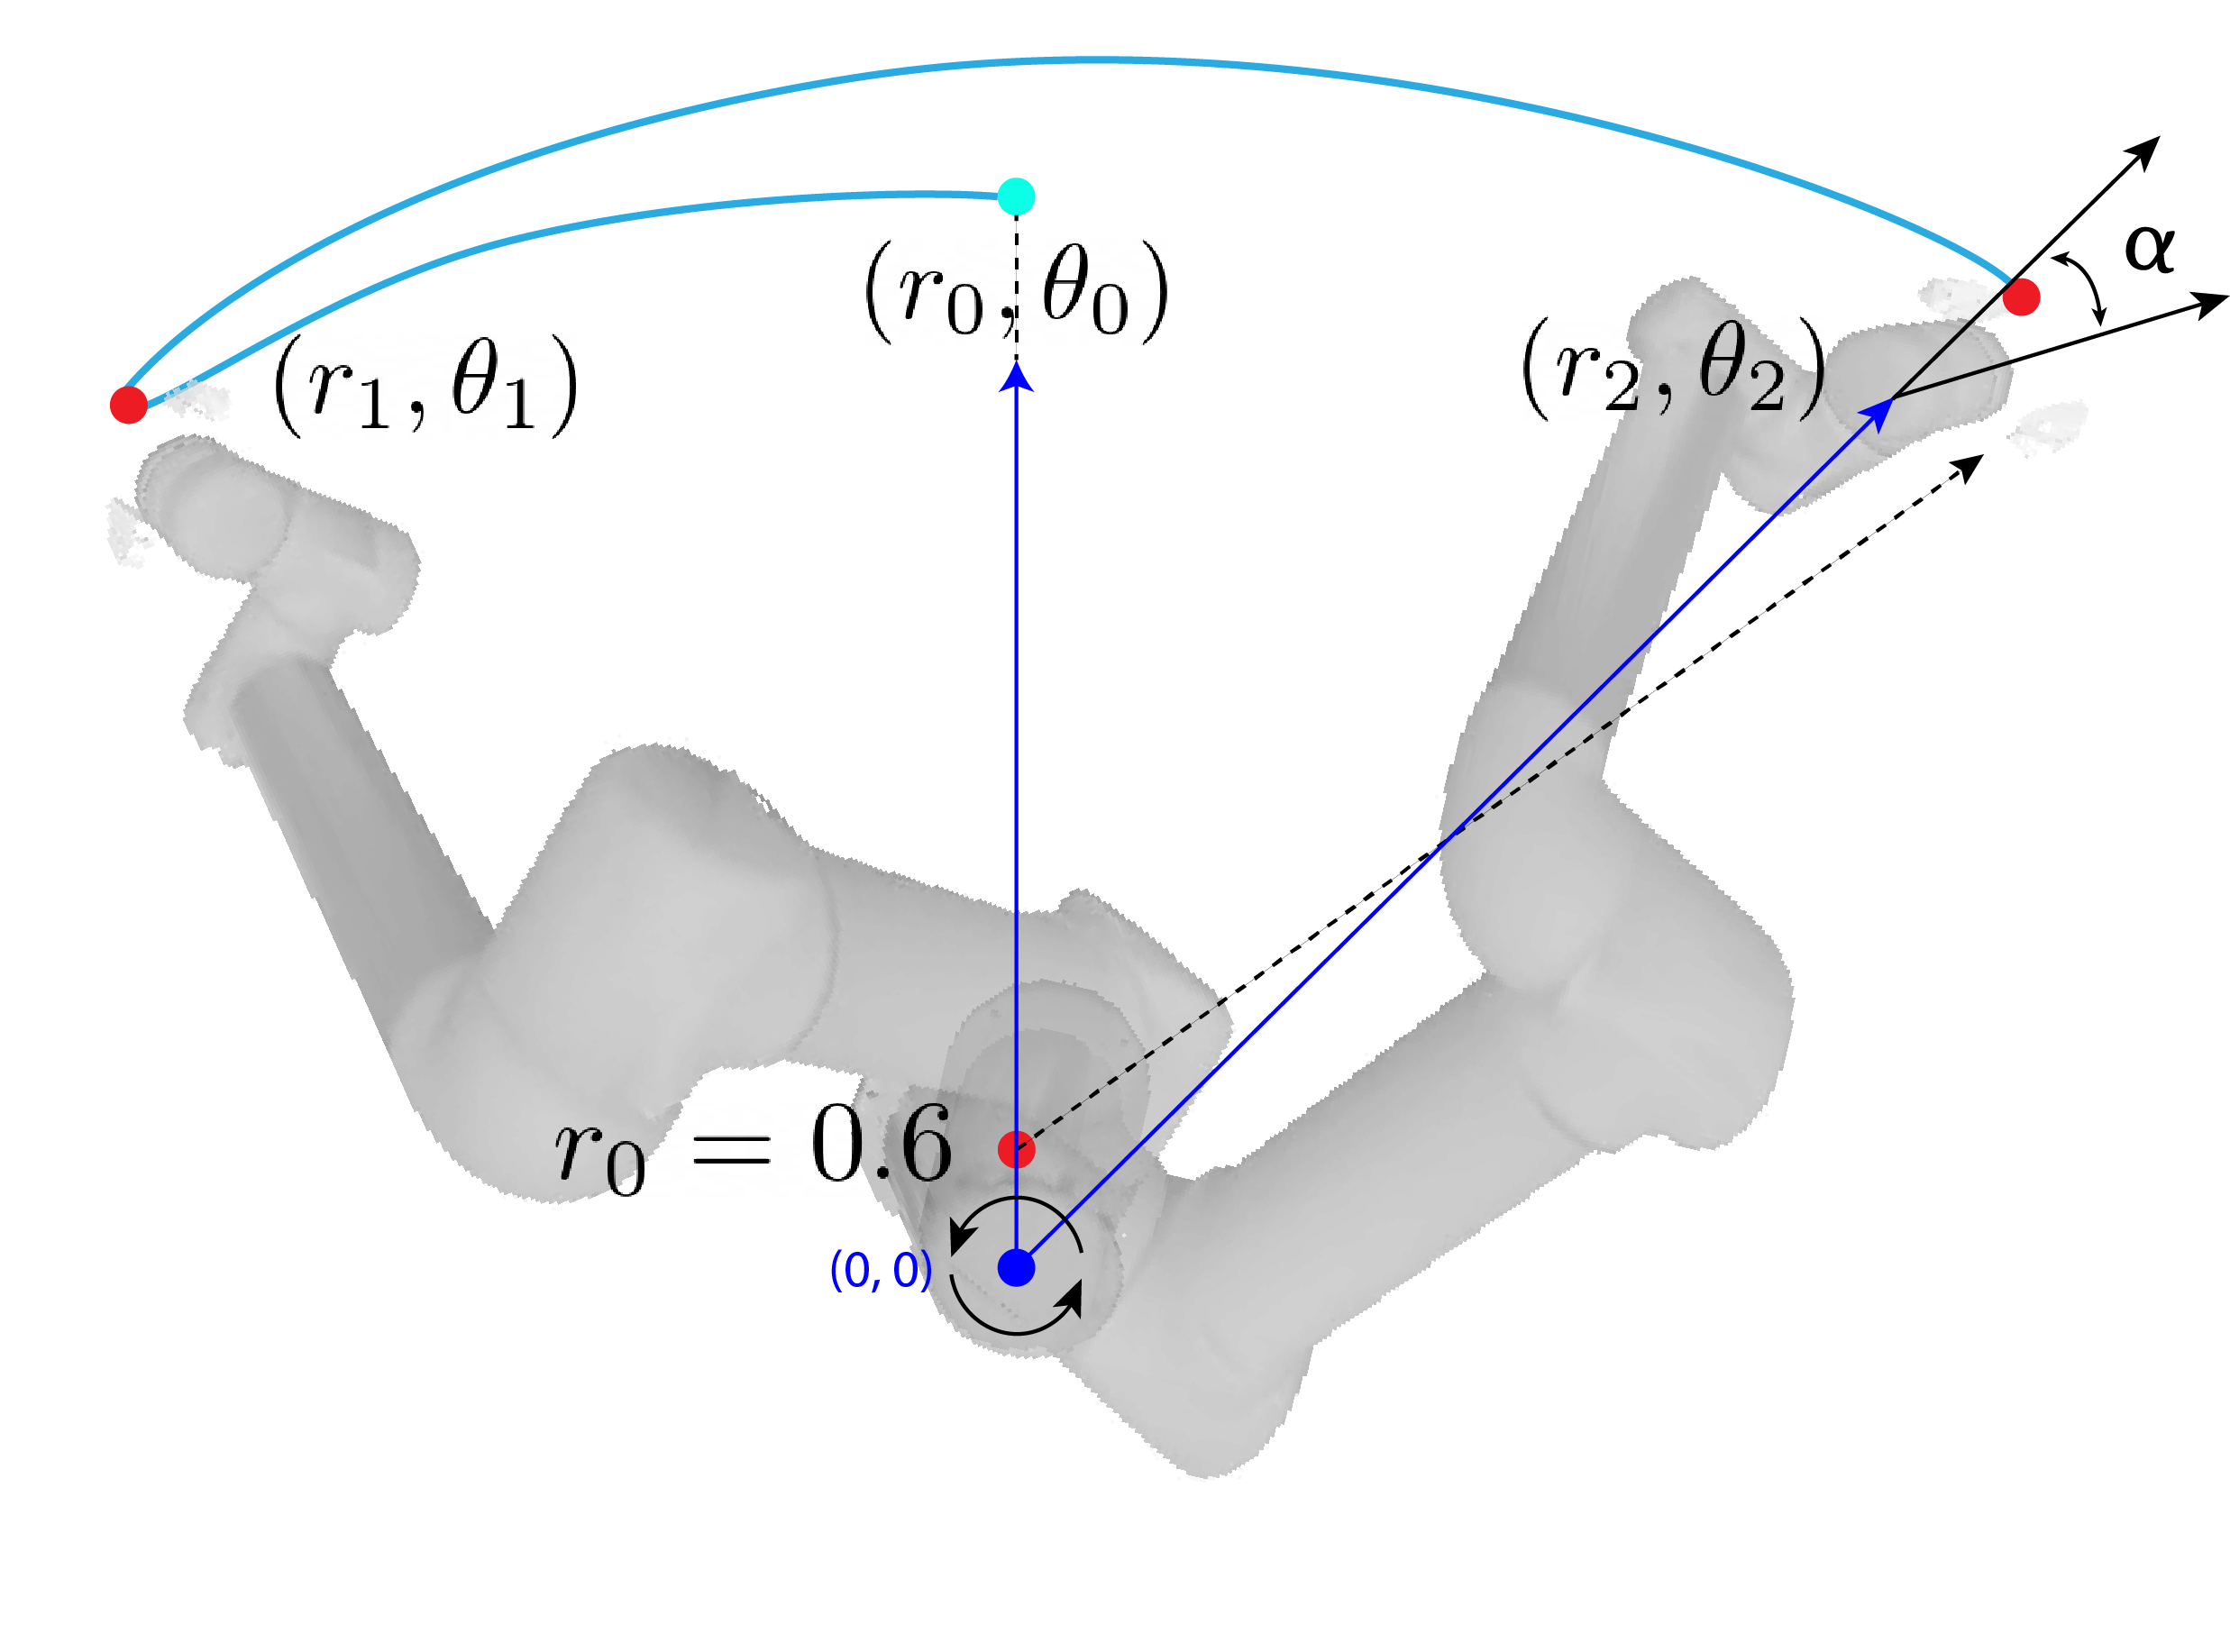
\includegraphics[width=0.33\textwidth]{figures/gif3l.png}
\vspace{-0.5cm}
\caption{
Example of a spline trajectory traced by the end effector of the UR5 for $r_0=0.6$. The reset procedure brings the end effector to $(r_0, 0)$ and the motion is smoothly interpolated along one spline to $(r_1, \theta_1)$, then along a second spline to $(r_2, \theta_2)$. Along the second spline, an offset $\alpha$ is added to the wrist joint angle produced by the IK solver.
}
\vspace*{-14pt}
\label{fig:spline}
\end{figure}

\subsection{Parameterized Actions}\label{ssec:action}

% \subsubsection{Parameterization}
% To generate dynamics actions that are quick and smooth; low-dimensional, thus facilitating data generation and training; and interpretable, we define a parameterized action composed of two sweeping arcs  (Fig.~\ref{fig:spline}):
To generate quick, smooth, dynamic actions that are low dimensional, thus facilitating data generation and training, we define a parameterized action $\ba := (\theta_1, r_1, \theta_2, r_2, \alpha, \vmax)$ composed of two sweeping arcs (Fig.~\ref{fig:spline}).
%We parameterize each action as:%by a vector of \emph{action variables}:
% \begin{equation}\label{eq:act1}
%     \ba = (\theta_1, r_1, \theta_2, r_2, \alpha, \vmax).
% \end{equation}
%The offset $r_0$ from the reset position is the origin of a polar coordinate frame. %Parameters $(\theta_1, r_1)$ and $(\theta_2, r_2)$ are the end-effector coordinates at the end of two successive arc motions (Fig.~\ref{fig:spline}). 
The motion starts at $(r_0, 0)$, arcs to $(r_1, \theta_1)$, and arcs back to $(r_2, \theta_2)$.
In the motion, $\alpha$ is the wrist joint rotation about the $z$-axis during the second arc, and $\vmax$ is the maximum velocity.
This parameterization is motivated by observing human attempts at the PRC task. %by doing motions arcing one direction opposite to the target position, then arcing back towards the target, before coming to a stop. During the motion, the human turns the wrist along the motion direction to increase the sweeping range of the cable. 

We convert action parameters to a trajectory in polar coordinates using a cubic spline to smoothly interpolate the radial coefficient from $r_0$ to $r_2$, and use a maximum-velocity spline to interpolate the angular coefficient from $0$ to $\theta_1$ and from $\theta_1$ to $\theta_2$, with maximum velocity $\vmax$. % The maximum-velocity spline uses a jerk-limited bang-bang control, having observed that the UR5 has difficulty following trajectories with high jerk~\cite{ichnowski2020djgomp}. 
The UR5 has difficulty following high-jerk trajectories, so the maximum-velocity spline uses jerk-limited bang-bang control~\cite{ichnowski2020djgomp}. We assume a direction change between the two arc motions, so the angular velocity at $\theta_1$ is 0. 
% \Vincent{I think we can cut this next equation for space.} By using this jerk-limited bang-bang control, we reduce the action parameterization to
% \begin{equation}\label{eq:act2}
%     \ba = (\theta_1, \theta_2, r_2, \alpha, \vmax).
% \end{equation} 
We use an analytic inverse kinematics (IK) solver to convert the splines to joint configurations. The execution for each trajectory is about 22 seconds, including  20 seconds for the reset motion and 2 seconds for the planar motion.

This parameterization enables state symmetry. For all datasets, we sample actions such that $\theta_1 > 0$, $\theta_2 < 0$, and $\alpha \geq 0$, to obtain targets on the left of the workspace axis of symmetry. If $(\theta_1, \theta_2, r_2, \alpha, \vmax)$ produces target $(r_d, \theta_d)$, $(-\theta_1, -\theta_2, r_2, -\alpha, \vmax)$ will produce $(r_d, -\theta_d)$. Thus, we do not evaluate targets on the right of the axis of symmetry.

% during evaluation, for targets $(r_d, \theta_d)$ on the left of the axis, we take $\pi((r_d, -\theta_d)) = (\hat{\theta}_1, \hat{\theta}_2, \hat{r}_2, \hat{\alpha}, \vmax)$ and output $(-\hat{\theta}_1, -\hat{\theta}_2, \hat{r}_2, -\hat{\alpha}, \vmax)$.

% \subsubsection{Repeatability}
% \Vincent{Perhaps cut this section as well since we don't put much emphasis on it.} \ale{Move this to the appendix} Highly non-deterministic trajectories will result in inconsistent simulator tuning results. We evaluate the repeatability of trajectories with respect to the $\vmax$ action parameter. We grid sample each parameter $(\theta_1, \theta_2, r_2, \alpha, \vmax)$ to generate $4\times4\times3\times3\times3$ trajectories for $\vmax \in \{2.0, 2.5, 3.0\}$ and run each trajectory 5 times on cable 1 to fix the $\vmax$ range. We find that with $\vmax \in \{2.0, 2.5\}$, the mean distance to the mean location of the 5 trials remains at 2\%, but with $\vmax=3.0$ the repeatability decreases with the mean distance to the mean location increasing to 4\%, so we limit $\vmax \leq 2.5$.

\subsection{Self-Supervised Physical Data Collection} \label{ssec:phys-data}

For the first step of R2S2R, we autonomously collect a physical dataset $\dreal$ and take a subset of $\dreal$ to form a simulator tuning dataset $\dtune$ to perform system identification in simulation (Sec.~\ref{ssec:sim-tuning}). % \Vincent{To fit into R2S2R pipeline, removed mentions of $\dsim$ until later.}
% To evaluate performance of policies learned only on real data, only simulation data, or a combined simulation and real dataset, 
% We collect two datasets for each cable: $\dreal$ and $\dsim$. Dataset $\dreal$ of size $N_1$ comes from physical experiments in real. We take a subset of trajectories from $\dreal$ to form a simulator tuning dataset $\dtune$ for performing system identification (see Section~\ref{ssec:sim-tuning}). We use the tuned simulation parameters to generate $\dsim$ of size $N_2$, where $N_2 \gg N_1$. We then use a combined dataset of $\dreal$ and $\dsim$ to train a policy for PRC.
% To create $\dtune$, we grid sample each parameter $(\theta_1, \theta_2, r_2, \alpha, \vmax)$ to generate $4\times4\times3\times3\times2$ trajectories, then filter it such that each trajectory abides by joint limits and is collision-free for a total of $N_1=90$ trajectories. 
To create $\dreal$, we grid sample each action parameter to generate $5{\times}5{\times}5{\times}4{\times}2$ trajectories, then filter out trajectories in collision or exceeding joint limits,
% it such that each trajectory abides by joint limits and is collision-free, 
to generate $|\dreal|=522$ trajectories. Refer to project website for grid sampling details. 
%\Lawrence{From our IROS reviewer: ``In V C, the paper writes “the execution for each trajectory is about 25s, including 15s for reset motion and 5s for planar motion, thus motivating the need for more efficient self-supervised data generation in simulation.” Why are these specific timings the motivation? What is more efficient self-supervised data generation in simulation? This is not clearly explained to me.''}

% As deformable objects are infinite-dimensional systems, we only track the cable endpoint. 
For automatic data labeling, we record each trajectory and use OpenCV contour detection  \cite{opencv_library} to track a brightly colored endpoint. We extract the 2D waypoint location $p_t = (x_t, y_t)$, where $t$ is the timestep, every 100\,ms from the start of the robot's trajectory. For each trajectory $m_j$ in $\dreal$, the number of waypoints collected is $K_j = \lfloor {T_j}/{100} \rfloor$, where $T_j$ is the duration of $m_j$ in milliseconds. 

\subsection{Three Simulation Models for Robot Casting}\label{ssec:simulators}

R2S2R then tunes a simulator to generate data to augment policy training. We consider which simulator and model best match real from 3 options: PyBullet~\cite{coumans2019} and two versions of NVIDIA Isaac Gym~\cite{makoviychuk2021isaac}.
We set simulated cable geometry (\eg length and radius) to match the real cable. Fig.~\ref{fig:sim_cables} shows a visual comparison, and the website provides further details.

\textbf{PyBullet} is a CPU-based deterministic rigid-body physics simulator used in prior work on deformable object manipulation~\cite{sim2real_deform_2018,seita_bags_2021}. We model the cable as a string of capsule-shaped rigid bodies with 6-DOF spring constraints between each consecutive pair. %as the adjustable angular stiffness values of these constraints can model twist and bend stiffness of cables.
We tune ten parameters: twist stiffness, bend stiffness, mass, lateral friction, spinning friction, rolling friction, endpoint mass, linear damping, angular damping, and dynamic friction. 

\textbf{NVIDIA Isaac Gym} is a GPU-based robotics simulation platform that supports the FleX~\cite{flex_2014} particle-based physics simulator designed for %fluids, cloths, cables, and other
deformable objects and rigid bodies. We test two simulation models for the cable: a \emph{segmented} model and a \emph{hybrid} model, both using Flex. 
The segmented model is a string of 18 capsule-shaped rigid bodies with consecutive pairs linked together by %3 hinge joints to simulate
a ball joint. To model cable stiffness, we tune the joint friction, cable mass, endpoint mass, and planar friction to capture variation in each respective parameter in real.
The hybrid model has the same rigid endpoint from the segmented model, but the rest of the cable is a soft-body rod. % modeled using tetgen~\cite{10.1145/2629697} to take advantage of soft-body simulation capabilities within FleX.
We tune the Young's modulus of the soft-body rod to model both the cable stiffness and elasticity, dynamic friction of the ground plane, and rigid endpoint mass to capture variations in friction and endpoint properties. Simulation environment details are on the website.


% Vincent: use this drawings:
% https://docs.google.com/drawings/d/1l8xT55nfJyCzjVjhFApZdNc45TuOtySqPDKsT6UghUc/edit?usp=sharing
\begin{figure}[t]
  \center
  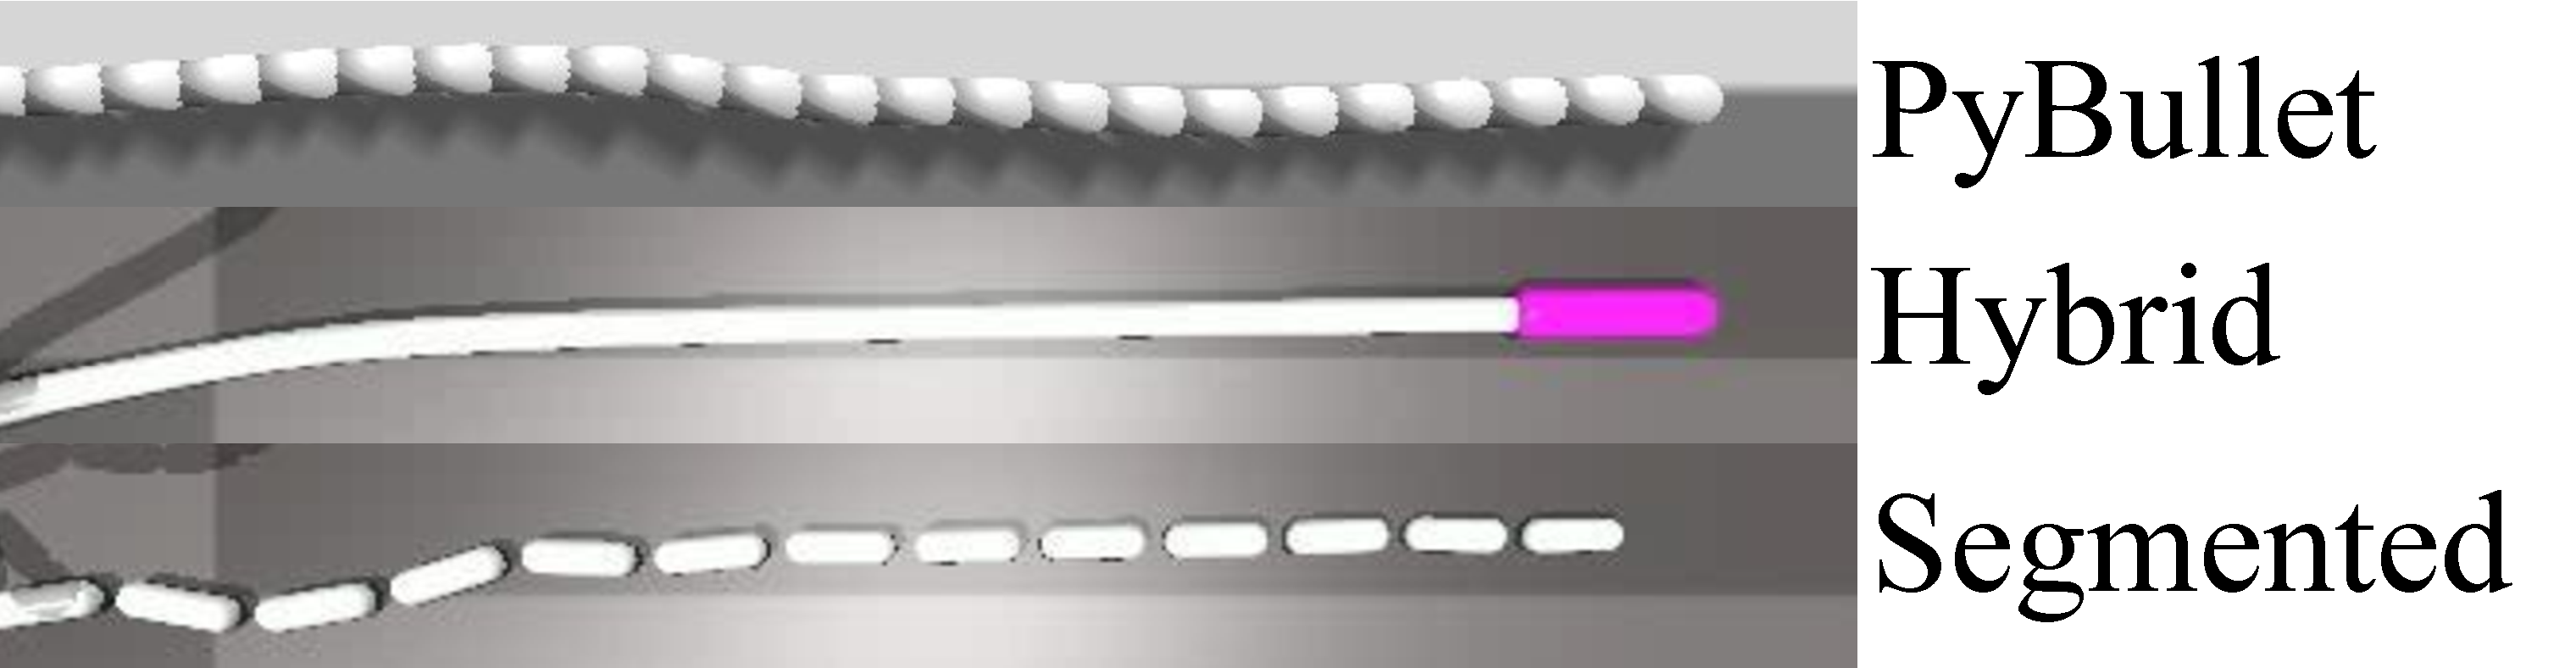
\includegraphics[width=0.46\textwidth]{figures/sim_fig_v2.pdf}
  \caption{
  Three cable simulation models for Real2Sim tuning. From top to bottom: the PyBullet model consists of capsule rigid bodies connected by 6 DOF spring constraints. The hybrid model is a soft-body rod connected to a capsule rigid body at the endpoint. The segmented model also consists of a string of capsule rigid bodies, but is connected using ball joints.
  }
  \vspace*{-14pt}
  \label{fig:sim_cables}
\end{figure}

% Only include if we have space.
% \Vincent{Should we include a blurb about the failed simulation models, e.g. the PhysX segmented model (too high non-determinism) or the segmented model in PyBullet (too unstable)?} \daniel{Low priority, only if room}

% Feel free to remove below
% ---
% We also attempted to simulate the cable with Incremental Potential Contact, a computer graphics simulator for softbodies with isotropic hyperelastic material model… (more description, will take from IPC-GraspSim paper). We initially hypothesized that its higher demonstrated fidelity in their paper would be an improved model of our ropes, since it could robustly handle different cable thicknesses and self-collisions occurring throughout the trajectory. However, the results were worse than the two primary simulators (we inspect $>100$\% average waypoint and endpoint errors). We observe a tradeoff between flexibility and stiffness/elasticity; we want our ropes to be flexible (small turning radius), but not elastic (cable should not drag on the floor). However, in this material model, it is difficult/impossible to do this since the model assumes an isotropic material. However, cable is a highly anistropic object (is good with shearing, but very resistant to stretching axially). In softbody simulation, although its inertia might initially get the cable configuration more similar to our desired physical position, its restorative forces (due to the stiffness parameters) force the mesh away and straighten out the mesh. Furthermore, the simulator was too slow (order of tens of seconds per simulation), making it not viable to perform a full parameter sweep.
% ---
% \raven{I think the following is not needed?}We additionally experimented three more cable simulation models that we did not move forward with: the ``segmented" model using the PhysX backend in NVIDIA Isaac Gym, but we observed very high non-determinism, leading to unreliable results; the ``segmented" model in PyBullet, but we observed high instability with dynamic actions \Vincent{Need to clarify `dynamic actions'}; and a ``soft" model in Isaac Gym, which is identical to the ``hybrid" model except that it does not have the rigid-body endpoint, but we observed much higher realism with the ``hybrid" model.
\subsection{Simulator Parameter Tuning for $\dsim$ collection}\label{ssec:sim-tuning}

To tune the parameters of each simulator so that simulated and real trajectories closely match, we follow system identification~\cite{sys_id} and employ a consistent protocol that uses physical trajectories from $\dtune$ (Sec.~\ref{ssec:phys-data}) to minimize the discrepancy between simulated and real trajectories. We define the simulation tuning objective as finding simulation parameters that minimize the average $L^2$ distance between the cable endpoint in simulation $\hat{p_t}$ to the target endpoint $p_t$ over all trajectory timesteps, averaged over a batch of trajectories. We call this metric the average waypoint error. 

As the simulation models may have parameters that have no physical analog, such as the joint friction in the segmented model, or have parameters that do not act similarly to their physical counterparts~\cite{9340852}, we choose tuning algorithms that make no assumptions about the underlying dynamics model. We evaluate two derivative-free black box optimization algorithms, Bayesian Optimization (BO) and Differential Evolution (DE). % , both of which are  methods. 

%\Vincent{For space, I'd remove these next two paragraphs and refer readers to tutorial papers.} 
BO builds a probabilistic surrogate model and uses an acquisition function that leverages the uncertainty in the posterior to decide where to query next~\cite{frazier2018tutorial}. BO has been used in policy search for RL hyperparameters~\cite{shahriari2015taking,lizotte2007automatic}, and for tuning simulation fluid dynamics~\cite{9340852}.
DE is an evolutionary population-based stochastic optimization algorithm widely used for global optimization of nondifferentiable, multi-modal, and nonlinear objectives~\cite{storn1997differential}. DE maintains a population of candidate solutions at each iteration and generates new candidates by combing each population member with another mutated population candidate member. It evaluates the fitness of the trial candidates to update the population of candidate solutions until convergence. DE has been shown to be effective at simulation parameter tuning~\cite{de_tuning_2020}.

We evaluate each algorithm via Sim2Sim tests. Using a fixed set of simulation parameters, we generate a small dataset of trajectories to tune randomly initialized simulators to test the effectiveness of DE and BO. We consider the discrepancy between ground truth and predicted simulation parameters and average waypoint error (see results in Sec.~\ref{ssec:sim2sim-results}). We then tune the simulator parameters for each simulation model to the physical data using the best performing tuning algorithm. We tune the simulator using the same process but with \emph{physical} trajectories from $\dtune$. 


\subsection{Size of Simulator Tuning Set $\dtune$}
We subsample 20 trajectories from $\dreal$ to generate dataset $\dtune$. We evaluated whether increasing the size of $\dtune$ would reduce the discrepancy between simulation and real using a test set of 30 random physical trajectories not in $\dreal$. We observed negligible difference in test errors between using 20 and 60 trajectories, but the latter require $2\times$ as long to tune on the hybrid and PyBullet models. Tuning with $|\dtune|=20$ trajectories did not lead to a significant speedup in the segmented model, therefore we held this value fixed. % We did not observe a speedup in the segmented model, so for consistency, we continued tuning with $|\dtune|=20$ trajectories. 

After tuning, R2S2R generates training data $\dsim$ by grid sampling $\theta_1$, $\theta_2$, $r_2$, $\psi$, and $\vmax$ to generate $15\times15\times15\times10\times2$ values for each respective parameter. We then filter out any trajectories that violate joint limits or with collisions to generate $|\dsim| = 21,450$ $(\ba, \bs)$ simulated trajectories.

\subsection{Policies}\label{ssec:method}

\begin{comment}
\subsection{Manual Reset and Repeat to Measure Repeatability}\label{sec:resets-repeat}

% \Lawrence{``From our IROS reviewer: The Reset procedures are described in both the Learning Framework section and Evaluation section. Is it used in both? It is still unclear to me why this is necessary and how is it used in both training and evaluation?''}

A prerequisite for dynamic planar manipulation of free-end cables to a given target is that actions corresponding to state transitions must be repeatable. This means the same action starting from the same state should lead into highly deterministic resulting state to make this problem tractable. 
% \Lawrence{``From our IROS reviewer: In IV A, the paper writes “A prerequisite for this
% problem is that actions corresponding to state transitions
% must be repeatable.” If I am not mistaken, this is stated
% without support or explanation. What is “this problem”? Why
% must the actions satisfy this property?''}
We design and parameterize trajectories with the goal of maximizing repeatability, which we measure by executing the same action $\ba$ multiple times and recording the variance in the final endpoint location. Each action always starts from the same \emph{reset} state for learning efficiency and higher repeatability. To get the cable into a reset state, the robot performs a sequence of trajectories that reliably places the cable into a consistent state. We find an open-loop sequence that includes lifting the cable off a surface and letting it hang until it comes to rest. This may be part of a reliable reset method, as it undoes torsion consistently with sufficient time. For further details, see Section~\ref{ssec:resets} and Fig.~\ref{fig:reset}.
\end{comment}

% \jeffi{TODO: explain what the policies do before how they work or how they're trained.}\Vincent{Is this right?}
% For the PRC task, we learn a policy that, given a target location $\bs_d$, outputs a dynamic arm action $\ba$ that minimizes the Euclidian distance between the target location $\bs_d$ and the executed trajectory endpoint location $\bs_f$.
\subsubsection{Forward Dynamics Model}
\label{sssec:supervised}

Due to the multi-modality between a target endpoint $\bs$ and valid actions $\ba$, we do not learn a policy that directly predicts $\ba$ given $\bs_d$. Instead, we learn a forward dynamics model $f_{\rm forw}$ that predicts $\bs$ given $\ba$, and interpolates to select an action. We parameterize $f_{\rm forw}$ using a fully connected neural network. 
Given a dataset $\mathcal{D}$ of $(\ba, \bs_f)$ trajectories, the neural network learns to predict $\bs_f$ given $\ba$ via standard supervised regression. During evaluation, the policy $\pi$ grid samples 67,500 input actions $\ba$ to form a set $\mathcal{A}$ of candidate actions. It then passes each action through the forward dynamics model $f_{\rm forw}$, which outputs the predicted endpoint location $(\hat{x}, \hat{y})$ in Cartesian space. Given a target endpoint $\bs_d$ (in polar coordinates), the policy selects the action that minimizes the Euclidean distance between the predicted endpoint $\bs_f$ and target endpoint $\bs_d$: $\pi(\bs) = \argmin_{\ba \in \mathcal{A}} \; \| \bs_{f, c} - \bs_{d, c} \|_2$, % the action ${\ba = \pi(\bs_d)}$ selected is the one minimizing the Euclidean distance between the predicted endpoint $\bs_f$ and the target endpoint $\bs_d$: $\pi(\bs) = \argmin_{\ba \in \mathcal{A}} \; \| \bs_{f, c} - \bs_{d, c} \|_2$,
% \begin{equation}\label{eq:finv}
% % \pi(\bs) = \argmin_{\ba \in \mathcal{A}} \; \| f_{\rm forw}(\ba) - g_{\rm p2c}(\bs) \|_2
% \pi(\bs) = \argmin_{\ba \in \mathcal{A}} \; \| \bs_{f, c} - \bs_{d, c} \|_2,
% \end{equation}
where $\state_{f, c}$ and $\state_{d, c}$ are $\state_f$ and $\state_d$ in Cartesian coordinates respectively. Training details can be found on the website. % \Vincent{Maybe the inverse dynamics model stuff should be in appendix too}
% We also attempted to learn an inverse dynamics model, which predicts $\ba$ given $\bs_d$ also via supervised regression, instead of a forward dynamics model, but we observed that the inverse model achieved much higher loss. We attribute this to the multi-modality between a target endpoint $\bs$ and valid actions $\ba$, while MSE loss typically assumes a unimodal regression target~\cite{mixture_density_networks}. 

\subsubsection{Baseline Policies}\label{sssec:baseline}

We consider two alternative policies:

\textbf{\polarcasting}. Given a target cable endpoint location $\bs_d = (r_d,\theta_d)$, the robot rotates $\theta_d$ radians and executes a rotated reset motion as in Sec.~\ref{ssec:resets}, causing the free endpoint to land at $(r, \theta_d)$. The robot then slowly pulls the cable toward the base for a distance of $r - r_d$. The robot arm is limited to a minimum $r$ coordinate of $r_{\rm min}=0.55$ to prevent the end effector from hitting the robot's supporting table, where $r_{\rm min}$ is the distance from the center of the robot base to the edge of the table, limiting the reachable workspace. 

\textbf{Forward Dynamics Model using Gaussian Process.} As a learning baseline, we train a GP regressor~\cite{Gaussian_process_ML,Mukadam_2018} using $\dreal$ to predict the cable endpoint location $\bs_f$ given input action $\ba$. As with the neural network forward dynamics model, we grid sample 67,500 input actions and select the trajectory that minimizes the predicted Euclidian distance to the target. We do not train a GP regressor using the simulated dataset as GP regression becomes intractable for large datasets with thousands of datapoints~\cite{belyaev2014exact}.

\section{Experiments}
\label{sec:experiments}

We evaluate the R2S2R pipeline on PRC with 3 cables (Fig.~\ref{fig:cables}) using a UR5 robot (Fig.~\ref{fig:teaser}).
The working surface is a \SI{2.45}{\meter} wide and \SI{1.55}{\meter} tall masonite board, painted blue and sanded to create a consistent friction coefficient across the surface. We use an overhead Logitech Brio 4K webcam recording 1920$\times$1080 images at 60 frames per second.

% We create three datasets for the cable: $\mathcal{D}_{\rm 1}$, real trajectories for tuning the simulator, $\mathcal{D}_{\rm 2}$, trajectories executed in the tuned simulator to train a policy $\pi$, and $\mathcal{D}_{\rm 3}$, real trajectories used for fine-tuning the policy trained on simulation examples. Using an overhead camera, we collect $N_1$ observations of actions and final state $\bs_f$ pairs to create $(\ba, \bs_f)$ data for $\mathcal{D}_1$. We then generate $N_2 \gg N_1$ simulated actions and $\bs_f$ pairs, to create $(\ba, \bs_f)$ data for $\mathcal{D}_2$. 


% Daniel: use this drawings:
% https://docs.google.com/drawings/d/13_Q0wpzHJVEir4x8EUV-o7NtrMx3G1IrJxrCZg-yr7o/edit?usp=sharing
% transparent version: https://docs.google.com/drawings/d/1eDjScikOTZQWP84CnQl2UZv1Kb2x7wtm7a7sGjDm6VY/edit?usp=sharing
\begin{figure}[t]
  \center
  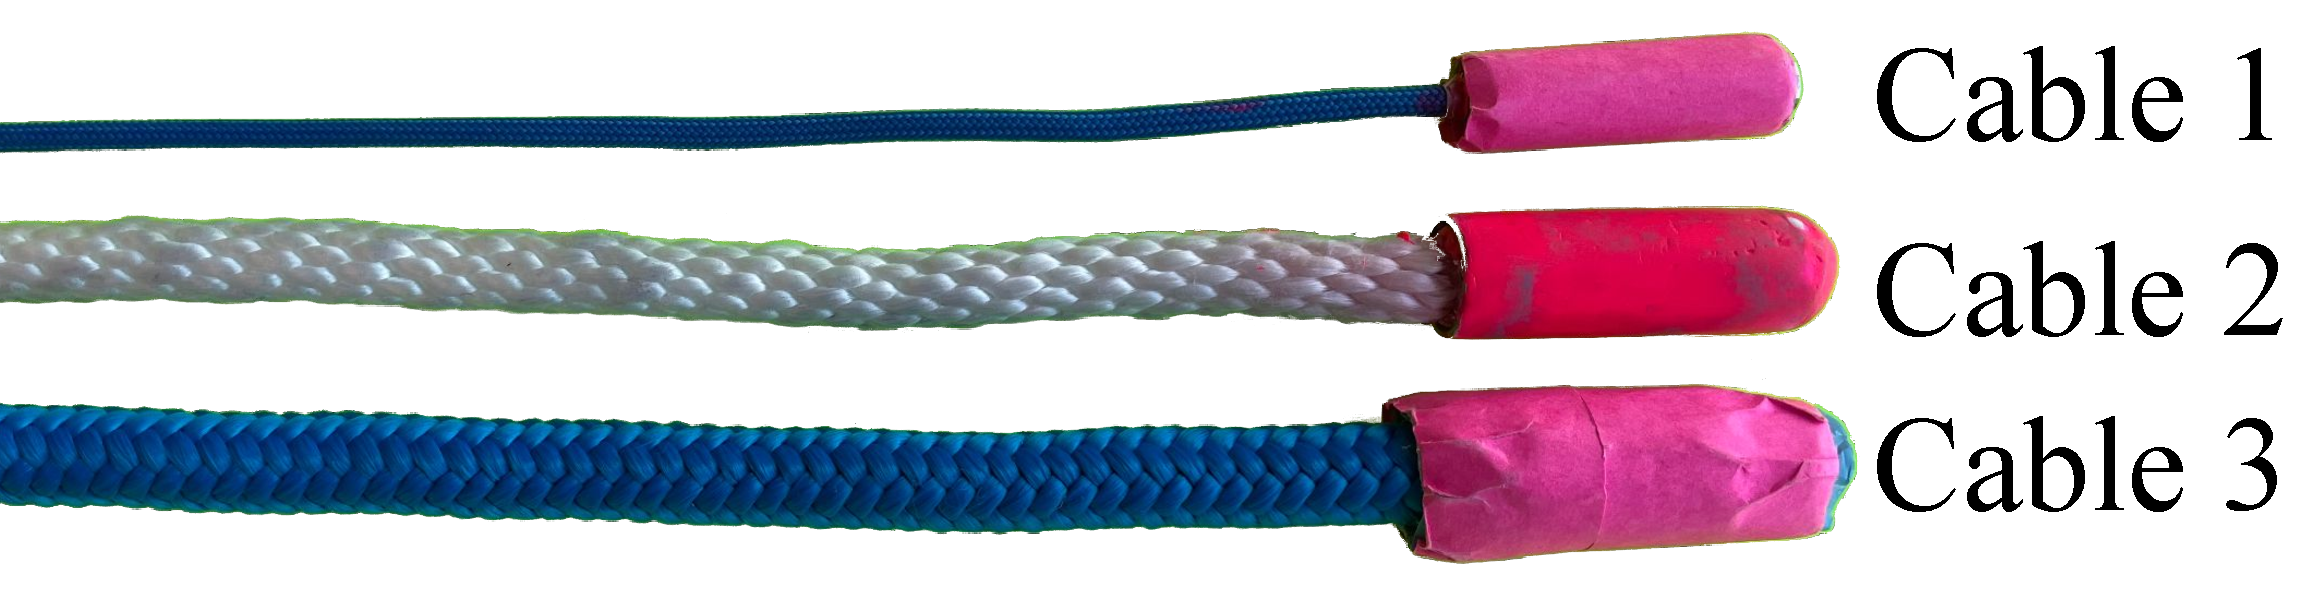
\includegraphics[width=0.45\textwidth]{figures/cables_v04_icra.pdf}
  \caption{
  Three cables used in physical experiments. Cable 1 is a thin blue paracord, Cable 2 is a nylon cable, and Cable 3 is a thick jump rope. Each endpoint has an attached mass. The respective cable lengths are \SI{0.63}{\meter}, \SI{0.65}{\meter}, and \SI{0.65}{\meter}, the respective masses are \SI{8}{\gram}, \SI{50}{\gram}, and \SI{45}{\gram}, and the respective radii are \SI{4.5}{\milli\meter}, \SI{10}{\milli\meter}, and \SI{14}{\milli\meter}.
  }
  \vspace*{-10pt}
  \label{fig:cables}
\end{figure}

\begin{table}[t]
  \setlength\tabcolsep{5.0pt}
%   \begin{adjustbox}{width=\columnwidth,center}
  \centering
  \footnotesize
  \begin{tabular}{@{}lrrrrrr@{}}
  \toprule
  & \multicolumn{2}{c}{Cable 1}  & \multicolumn{2}{c}{Cable 2} & \multicolumn{2}{c}{Cable 3}\\
  \cmidrule(lr){2-3} \cmidrule(lr){4-5} \cmidrule(l){6-7}
  Sim. Model  & Wayp. & Last & Wayp. & Last & Wayp. & Last \\
  \midrule
  PyBullet         & 29\%  & 28\% & 28\%  & 28\%  & 23\% & 17\% \\
  Isaac Gym Hybrid & 14\%  & 23\% & 11\%  & 14\%  & 11\% & 13\%\\
  Isaac Gym Segm.  & \textbf{9\%} & \textbf{13\%} & \textbf{8\%}  & \textbf{9\%}  & \textbf{11\%} & \textbf{13\%}\\
  \toprule
  \end{tabular}
%   \end{adjustbox}
  \caption{
  Error for simulators tuned using DE on a set of 30 test trajectories for 3 cables (see Fig.~\ref{fig:cables}). The two metrics are the median final $L^2$-distance, which is the 2D Euclidean distance between endpoint locations in simulation and reality after a trajectory terminates, and average waypoint (``Wayp.'') error. Values are expressed in percentages of cable length.
  }
  \vspace*{-10pt}
  \label{tab:tuning}
\end{table}  

We consider three forward dynamics model policies:
\begin{enumerate}
    \item $\pireal$, trained on a small real dataset $\dreal$,
    \item $\pisim$, trained on a large simulated dataset $\dsim$,
    \item $\pitune$, trained on the combined dataset $\dreal \cup \dsim$.
\end{enumerate}
Since $|\dsim| \gg |\dreal|$, we 1) upsample $\dreal$ by randomly duplicating samples such that the real data make between 30\% and 40\% of the combined dataset to force the model to learn more from the real data, and 2) weight the loss function so that samples from $\dreal$ are weighted higher. We empirically choose the upsampling percentage and real sample weights to be the best performing values. 
% We experimentally show that the upsampled real dataset and weighted loss will help overcome the data distribution imbalance between the simulated and real data.


\begin{figure*}[!h]
    \centering
    % 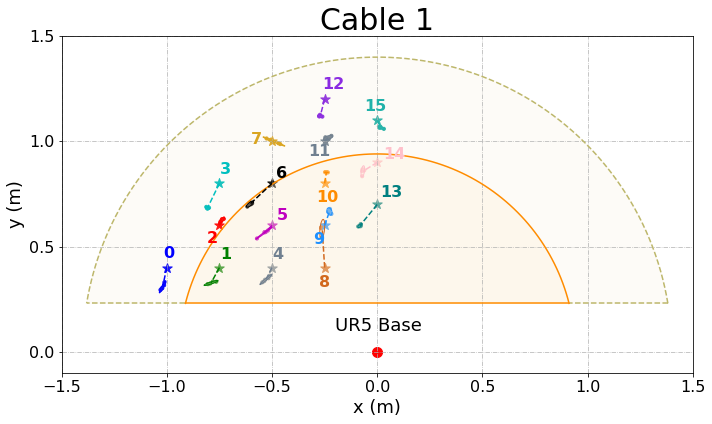
\includegraphics[width=0.32\textwidth]{figures/nylon.png}
    % 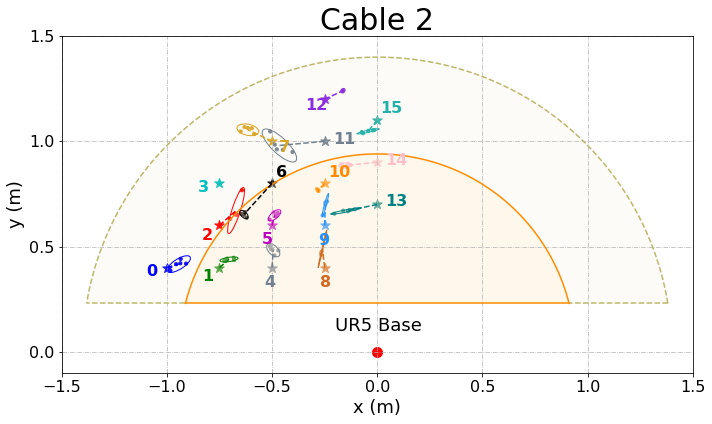
\includegraphics[width=0.32\textwidth]{figures/paracord.png}
    % 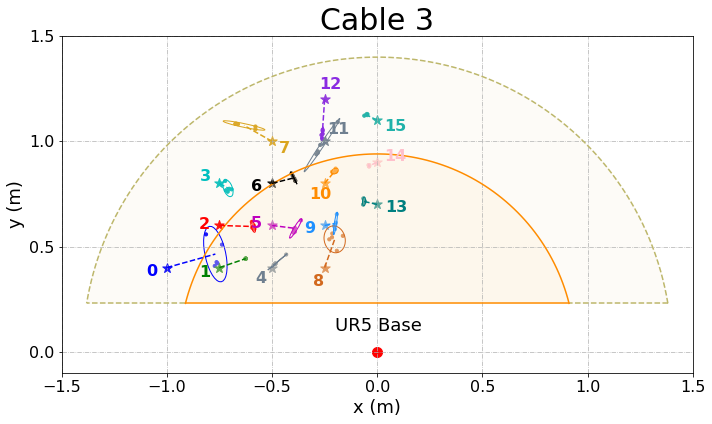
\includegraphics[width=0.32\textwidth]{figures/jump.png}
    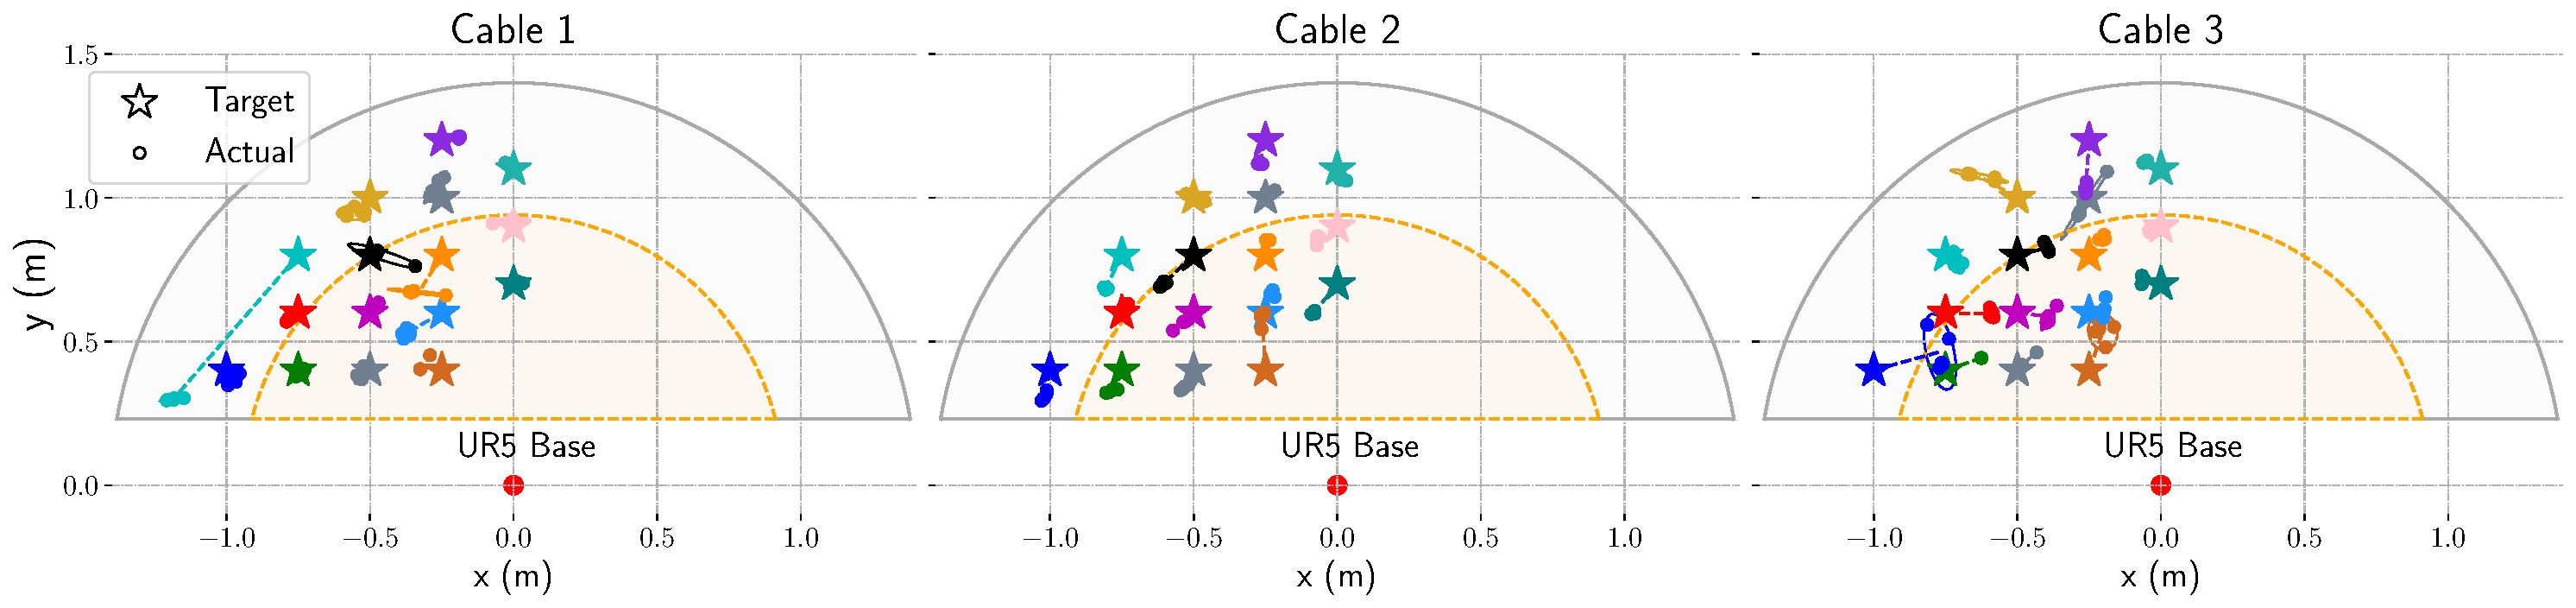
\includegraphics[width=\textwidth]{figures/error_plots_v3.pdf}
    \caption{
    Evaluation results for $\pitune$ for each cable. The inner orange shaded region represents the robot workspace and the outer grey shaded region represents the cable workspace.
    The colored stars and dots represent each of 16 target locations and resulting endpoints for 5 trials per target respectively, with associated 95\% confidence ellipses. The dashed lines connect the center of each ellipse to the target location representing the mean error in position. 
}
\label{fig:repeat_multi_cable}
\vspace*{-10pt}
\end{figure*}

\subsection{Comparing Real2Sim Tuning Methods}\label{ssec:sim2sim-results}
To test the effectiveness of BO and DE for tuning the Isaac Gym simulators, we generate simulated data for several hybrid models and segmented models with arbitrarily chosen parameters. We then apply BO and DE to tune the respective simulator model parameters.
For BO, we use the GPyOpt~\cite{gpyopt2016} library, and test three acquisition functions: Expected Improvement (EI), Lower Confidence Bound (LCB), and Maximum Probability of Improvement (MPI).
We use DE as implemented in SciPy~\cite{2020SciPy-NMeth}.
With 5 tuning trajectories, EI performs better than LCB and MPI. The tuning errors using BO range from 3.39\% to 17.98\% for the hybrid model and 1.09\% to 9.25\% for the segmented model. DE consistently tunes the parameters to within $1\%$ of the ground truth parameters for both the hybrid and segmented models, thus we use DE for all further simulator tuning results.

\subsection{Real2Sim}\label{ssec:real2sim-results}
Table~\ref{tab:tuning} reports the Real2Sim simulator tuning results using DE. We observe that the segmented model consistently outperforms the PyBullet and hybrid models in minimizing the discrepancy between simulation and real. For the hybrid model, We find that the tuning algorithms reduce the value of Young's modulus to decrease cable stiffness, but also increases the stretchiness along the length of the cable, which we did not observe in real. We attribute the PyBullet model performance to spring-system simulation instability associated with high spring forces, particularly when preventing the cable from stretching along the length of the cable.

For cable 3, we observe that the hybrid and segmented models perform similarly. Since cable 3 is stiffer, DE produces higher Young's modulus values that both make the simulated cable stiffer and cause it to stretch less along its length, both of which are desired properties.

While the errors for cable 2 are below 10\%, we observe that cables 1 and 3 are harder for each simulator to model, each with a 4\% higher last endpoint error for the segmented model. This may be due to plastic deformation in cables 1 and 3, as we observed that slight bends in the cables would remain until manually straightened by a human operator. We generate $\dsim$ using the segmented model, which requires approximately 4.5 minutes using 4 NVIDIA V100s.

% Daniel: move to top.
\begin{table}[t]
  \setlength\tabcolsep{5.0pt}
  \centering
  %\vspace{-1em}
  \vspace{1pt}
%  \begin{adjustbox}{width=\columnwidth,center}
  \centering
  \scriptsize
  \begin{tabular}{@{}lcrrrrr@{}}
  \toprule
  Model & Dataset & Median & $Q_1$ & $Q_3$ & Min & Max \\
  \midrule
  \polarcasting & N/A & 61\% & 38\% & 86\% & 6\% & 124\%\\
  Gaussian Proc. & $\dreal$ & 27\%  & 9\%   & 51\% & 4\% & 97\%\\
  $\pireal$ & $\dreal$ & 15\% & 11\% & 21\% & 8\% & \textbf{36\%}\\
  $\pisim$ & $\dsim$ & 14\% & 10\% & 17\% & 6\%& 115\%\\
  $\pitune$ & $\dreal \cup \dsim$ & \textbf{8\%} &\textbf{5\%} & \textbf{12\%} & \textbf{2\%} & 105\% \\
  \toprule
  \end{tabular}
  

    \caption{
    Physical evaluation results on Cable 1 of the 2 baselines and the dynamics model $f_{\rm forw}$ trained on three different datasets over a total of $16\times5=75$ trials. $Q_1$ and $Q_3$ are the first and third quartile. All errors are expressed as a percentage of cable length (\SI{0.65}{\meter}).
  }
  \label{tab:error}
  \vspace*{-5pt}
\end{table}
\subsection{Physical Experiments}
\label{ssec:physical-evaluation}

% Daniel: let's put tables at the top of the page.
\begin{table}[t]
  \setlength\tabcolsep{5.0pt}
  %\vspace{-1em}
  \centering
   \small
   %\begin{adjustbox}{width=\columnwidth,center}
     \centering
   \begin{tabular}{@{}lrrrrr@{}}
   \toprule
   Cable      & Median & 1st Quartile & 3rd Quartile  & Min & Max   \\
   \midrule
   Cable 1   & 8\% & 5\% & 12\% & 2\% & 105\% \\
   Cable 2   & 12\% & 8\% & 16\%& 4\% & 28\%\\
   Cable 3   & 14\% & 9\% & 23\% & 6\% & 38\% \\
   \toprule
   \end{tabular}
   %\end{adjustbox}
   \caption{
  Physical evaluation results using $\pitune$ of 3 cables (see Fig.~\ref{fig:cables}) on 16 target locations with 5 trials each per cable for a total of 75 trials using policies trained according to $\pitune$. All errors are expressed as percentages of cable length.
   }
   \vspace{-14pt}
  \label{tab:results}
\end{table}

As summarized in Table \ref{tab:error}, we evaluate two baseline policies and PRC policies $\pireal$, $\pisim$, $\pitune$ on cable 1. 
\subsubsection{Baseline Policies} The analytic ``\polarcasting'' baseline performs the worst out of any of the policies, as the robot would collide with the base for targets near the base. The GP trained on $\dreal$ has substantially worse median, 3rd quartile, and maximum errors, but slightly outperforms $\pireal$ in minimum and 1st quartile errors.
\subsubsection{Forward Dynamics Models} We find that policies $\pireal$ and $\pisim$ have similar median and first and third quartile errors, but $\pisim$ has a substantially higher maximum error, corresponding to trajectories where the simulator has high tuning error.
As the simulator is tuned with only 20 trajectories, compared to the over 500 trajectories used to train $\pireal$, we achieve similar evaluation performance while using 96\% fewer physical trajectories. When we combine the two datasets to train $\pitune$, the median error drops by nearly 50\%. The maximum error rose to above 100\% for a single target, suggesting that while the combined dataset substantially improves overall results, it may introduce outliers in regions of the workspace with high reality gap. 
Given that $\pitune$ performs the best out of the policies, we proceed to evaluate the performance for 3 cables on 16 target positions using policy $\pitune$ trained for each cable separately, and repeat each action 5 times per target. Results are summarized in Table~\ref{tab:results}. We quantify the aleatoric uncertainty with the 95\% confidence ellipses in Fig.~\ref{fig:repeat_multi_cable}. 

We attribute the epistemic uncertainty to two sources: the Sim2Real gap, where trajectories executed in simulation do not accurately reflect real, and the learning error in the forward dynamics model. The results suggest that the R2S2R pipeline can apply to other cables.


\section{Conclusion and Future Work}\label{sec:conclusion}

In this paper, we present Real2Sim2Real, a self-supervised learning framework, and apply it to Planar Robot Casting. Experiments suggest that the framework, which collects physical data, tunes a simulator to match the real data, and trains policies from a weighted combination of real and simulated data, can achieve an median error between 12\% and 15\% of cable length on the PRC task.

As motion is restricted to a 2D plane, we do not address the 3D analog of PRC, Spatial Robot Casting (SRC), used in tasks such as fly fishing~\cite{fly_fishing_2004}. PRC is easier to visualize than SRC but can be harder to model due to inherent uncertainty about static and dynamic friction. In both PRC and SRC, the cable is infinite-dimensional and there is a long time horizon for the motion of the cable free end resulting from a motion at the controlled end. 

In future work, we will explore alternate Real2Sim and Sim2Real techniques~\cite{auto-tune_2021,allevato2020tunenet,Fox-RSS-19,dynamics_randomization_2018} and apply Real2Sim2Real to other tasks such as grasping and fabric manipulation.
% Daniel: don't make this tiny font.
% IMPORTANT ADD BACK FOR FINAL PRINT VERSION!!!!
\section*{Acknowledgments}

{\footnotesize
This research was performed at the AUTOLAB at UC Berkeley in affiliation with the Berkeley AI Research (BAIR) Lab and the CITRIS ``People and Robots'' (CPAR) Initiative. The authors were supported in part by the Toyota Research Institute. We thank our colleagues Justin Kerr, Alejandro Escontrela, Ashwin Balakrishna, Ellen Novoseller, Brijen Thananjeyan, Harry Zhang, Zachary Tam, Chung Min Kim, and Ananth Rao for helpful comments.
}


% \clearpage Daniel: can do this if needed
%\footnotesize
% \bibliographystyle{IEEEtranS}
% \bibliography{example}
\renewcommand*{\bibfont}{\footnotesize}
\printbibliography

% Back to normal size.
%\normalsize
% \cleardoublepage
% \appendix
% %%%%%%%%%%%%
% APPENDIX %
%%%%%%%%%%%%
\section{Appendix}\label{app}
The appendix is structured as follows:

\begin{itemize}
    \item In Appendix~\ref{app:isaac-gym} we provide more background on NVIDIA Isaac Gym 
    \item In Appendix~\ref{app:method-details} we provide more details on the methodology.
\end{itemize}


\subsection{NVIDIA Isaac Gym}\label{app:isaac-gym}

We use the Flex physics engine in Isaac Gym. With the Flex backend, we use the Newton Jacobi solver for its determinism guarantees to ensure consistent Real2Sim tuning results. We use a simulation timestep of 1/60\,s with 8 substeps, 5 inner iterations, and 20 outer iterations, and did not observe these parameters to affect the determinism. However, we observed that increasing the granularity of these parameters to increase simulation stability and fidelity results in substantially increased runtime. As such, we minimized these parameters to the extent permitting stability.

For the Isaac Gym segmented model, the cable has 18 rigid links connected by ball joints. We tried increasing the number of links up to a maximum of 30 and noticed insignificant increase in simulation fidelity, but a significant decrease in simulation fidelity. As the rigid links are connected by ball joints, the segmented model should be unable to model stretching along the length of the cable. However, we noticed stretching along the length of the cable in as we increased the number of rigid links, which we interpreted as a sign of simulation instability and opted to decrease the number of rigid links.  

\subsection{Additional Method Details}\label{app:method-details}

For policy $\pireal$, we parameterize the forward dynamics model $f_{\rm forw}$ with a feedforward neural network with 3 layers, each with 32 hidden units, and mini-batch size of 16. For policies $\pisim$ and $\pitune$, we parameterize $f_{\rm forw}$ with a larger neural network with 3 layers, each with 128 hidden units, and a mini-batch size of 64. We use a smaller neural network for $\pireal$ to avoid overfitting to the small real dataset, whereas $\pisim$ and $\pitune$ both train on larger, more diverse datasets. For all policies, we use the Adam optimizer~\cite{adam2015} and a learning rate of $10^{-3}$.

For each policy, we train the neural network to minimize the predicted $L^2$ loss for each $(\ba, \bs)$ data sample. For $\pisim$, we weight $\dreal$ samples 2$\times$ higher for cable 1, and 3$\times$ higher for cable 2, and $2\times$ higher for cable 3. We additionally tested upsampling percentages of between 20\% and 50\%, and picked values between 30\% and 40\%. These hyperparameters were chosen empirically to maximize performance. 

For grid sampling of the five trajectory parameters, the bounds for $\dreal$ are shown in Table~\ref{tab:dphys_samp}. The bounds were chosen to empirically maximize coverage of the reachable workspace.

\begin{table}[H]
  \setlength\tabcolsep{5.0pt}
  \centering
  \normalsize
  \begin{tabular}{@{}lccc@{}}
  \toprule
  Parameter & Lower & Upper & Frequency \\
  \midrule
  $\theta_1$ & \ang{1} & \ang{80} & 5 \\
  $\theta_2$ & \ang{20} & \ang{80} & 5 \\
  $r_2$ & 0.21 & 0.77 & 5 \\
  $\alpha$ & \ang{30} & \ang{60} & 4 \\
  $\vmax$ & 2 & 2.5 & 2 \\
  \toprule
  \end{tabular}
  \caption{$\dreal$ grid sampling ranges.}
  \label{tab:dphys_samp}
\end{table}

The grid sampling bounds for $\dsim$ is similar, with the only difference being the sampling frequency and the bounds for $\theta_2$, as shown in Table~\ref{tab:dsim_samp}.

\begin{table}[H]
  \setlength\tabcolsep{5.0pt}
  \centering
  \normalsize
  \begin{tabular}{@{}lccc@{}}
  \toprule
  Parameter & Lower & Upper & Frequency \\
  \midrule
  $\theta_1$ & \ang{1} & \ang{80} & 15 \\
  $\theta_2$ & \ang{1} & \ang{80} & 15 \\
  $r_2$ & 0.21 & 0.77 & 15 \\
  $\alpha$ & \ang{30} & \ang{60} & 5 \\
  $\vmax$ & 2 & 2.5 & 2 \\
  \toprule
  \end{tabular}
  \caption{$\dsim$ grid sampling ranges.}
  \label{tab:dsim_samp}
\end{table}

For tuning with Differential Evolution, we use the default parameters as implemented by SciPy~\cite{2020SciPy-NMeth}.

\subsection{Cable Model Parameters} \label{app:cable}

\Vincent{TODO}
\end{document}
